\documentclass{article}
\usepackage{../csci-246-fall2018/hw/template/fasy-hw}
\usepackage{amsmath}
\usepackage{cancel}

\author{Nathan Stouffer}
\problem{1-1}
% \problem{A-B} means Problem Set A, Problem B.
\collab{Kevin Browder and Cameron Blegen}
% or give names, e.g., \collab{Alyssa P. Hacker and A. Student}

\begin{document}

\section*{Section 4.3, Problem 33}
Question: Is it possible to have a combination of nickels, dimes, and quarters that add up to \$4.72?
\\\\
Proof: Let $n$ be the number of nickels, $d$ be the number of dimes, and $q$ be the number of quarters in 
\begin{center}
	(1) $472=5n+10d+25q$
\end{center}
It would be nonsensical to have non-integer values for $n,d,q$ because the variables represent coins, therefore $n,d,q\in\mathbb{Z}$. However, there is no integer solution to (1) because the equation can be manipulated to have only integers on one side and and non-integers on the other:
\begin{center}
	$472=5n+10d+25q$\\
	$472=5(n+2d+5q)$\\
	$\dfrac{472}{5}=n+2d+5q$
\end{center}
$\dfrac{472}{5}$ is a not an integer because $475$ $mod$ $5=2\neq0$. Therefore, if $n,d,q\in\mathbb{Z}$, the two sides of the equation can not be equal and there are no integer solutions to (1).

\section*{Section 4.3, Problem 34}
Question: Is it possible to have 50 coins, made up of pennies, dimes, and quarters, that add up to \$3?
\\\\
Proof: Let $p$ be the number of pennies, $d$ be the number of dimes, and $q$ being the number quarters. To satisfy the question, $p,d,q\in\mathbb{Z}$ and the following equations must be true:
\begin{center}
	(1) $300=1*p+10*d+25*q$\\
	(2) $50=p+d+q$
\end{center}
Equation (2) can be rearranged to isolate $p$ ($p=50-d-q$) and substitute (2) into (1) to form:
\begin{center}
	(3) $300=1*(50-d-q)+10d+25q$
\end{center}
Equation (3) can be simplified:
\begin{center}
	$300=1*(50-d-q)+10d+25q$\\
	$300=50-d-q+10d+25q$\\
	$250=9d+24q$\\
	$250=3(3d+8q)$\\
	$\dfrac{250}{3}=3d+8q$
\end{center}
$\dfrac{250}{3}$ is a not an integer because $250$ $mod$ $3=1\neq0$. Therefore, if $p,d,q\in\mathbb{Z}$, the two sides of the equation can not be equal and there are no integers $p,d,q$ that satisfy both (1) and (2).

\problem{1-2}
\collab{Kevin Browder}
\clearpage
\header

\section*{Section 4.4, Problem 15}
Question: January 1, 2000, was a Saturday, and 2000 was a leap year. What day of the week will January 1, 2050, be?
\\\\
Proof: Let $y$ be the current year for $y\geq2000$. If leap years did not exist, January 1st would advance one day of the week each year. An equation representing the day of the week where 0 corresponds to Sunday, 1 to Monday, ... and 6 to Saturday would be:
\begin{center}
	(1) $(y-2000)$ $mod$ $7$
\end{center}
The only missing component involves leap years. The leap years occur every 4 years beginning in 2000, adding this into the equation results in:
\begin{center}
	(2) $((y-2000) + (y-1997)//4)$ $mod$ $7$
\end{center}
where $//$ truncates the dividend $(y-1997)$ to form an integer and, for any $y\geq2000$, equation (2) represents the number of days past Saturday that January 1 is for that $y$. Plugging in $y=2050$:
\begin{center}
	$((2050-2000) + (2050-1997)//4)$ $mod$ $7$\\
	$(50 + 53//4)$ $mod$ $7$\\
	$(50 + 13)$ $mod$ $7$\\
	$63$ $mod$ $7$\\
	$0$
\end{center}
Therefore, January 1, 2050 will be the same day as January 1, 2000: Saturday.

\problem{1-3}
\collab{Kevin Browder}
\clearpage
\header

\section*{Section 4.4, Problem 35}
Question: Prove that any integer to the fourth power can be written as $8m$ or $8m+1$ for a particular $m\in\mathbb{Z}$.
\\\\
Proof: Let $n\in\mathbb{Z}$. Any $n$ can be written as $2q$ or $2q+1$ for $q\in\mathbb{Z}$. If $n=2q$:
\begin{center}
	\begin{align*}
		n^4&=8m\\
		(2*q)^4&=\\
		16*q^4&=\\
		8*(2*q^4)&=\\
		8m&=8m
	\end{align*}
\end{center}
Otherwise, $n=2q+1$:
\begin{center}
	\begin{align*}
		n^4&=8m+1\\
		(2q+1)^4&=\\
		16*q^4+32*q^3+24*q^2+8*q+1&=\\
		8*(2*q^4+4*q^3+3*8*q^2+q)+1&=\\
		8m+1&=8m+1
	\end{align*}
\end{center}

\problem{1-4}
\collab{Kevin Browder}
\clearpage
\header
\graphicspath{ {map_image} }
\begin{figure}[h]
	\centering
	\fbox{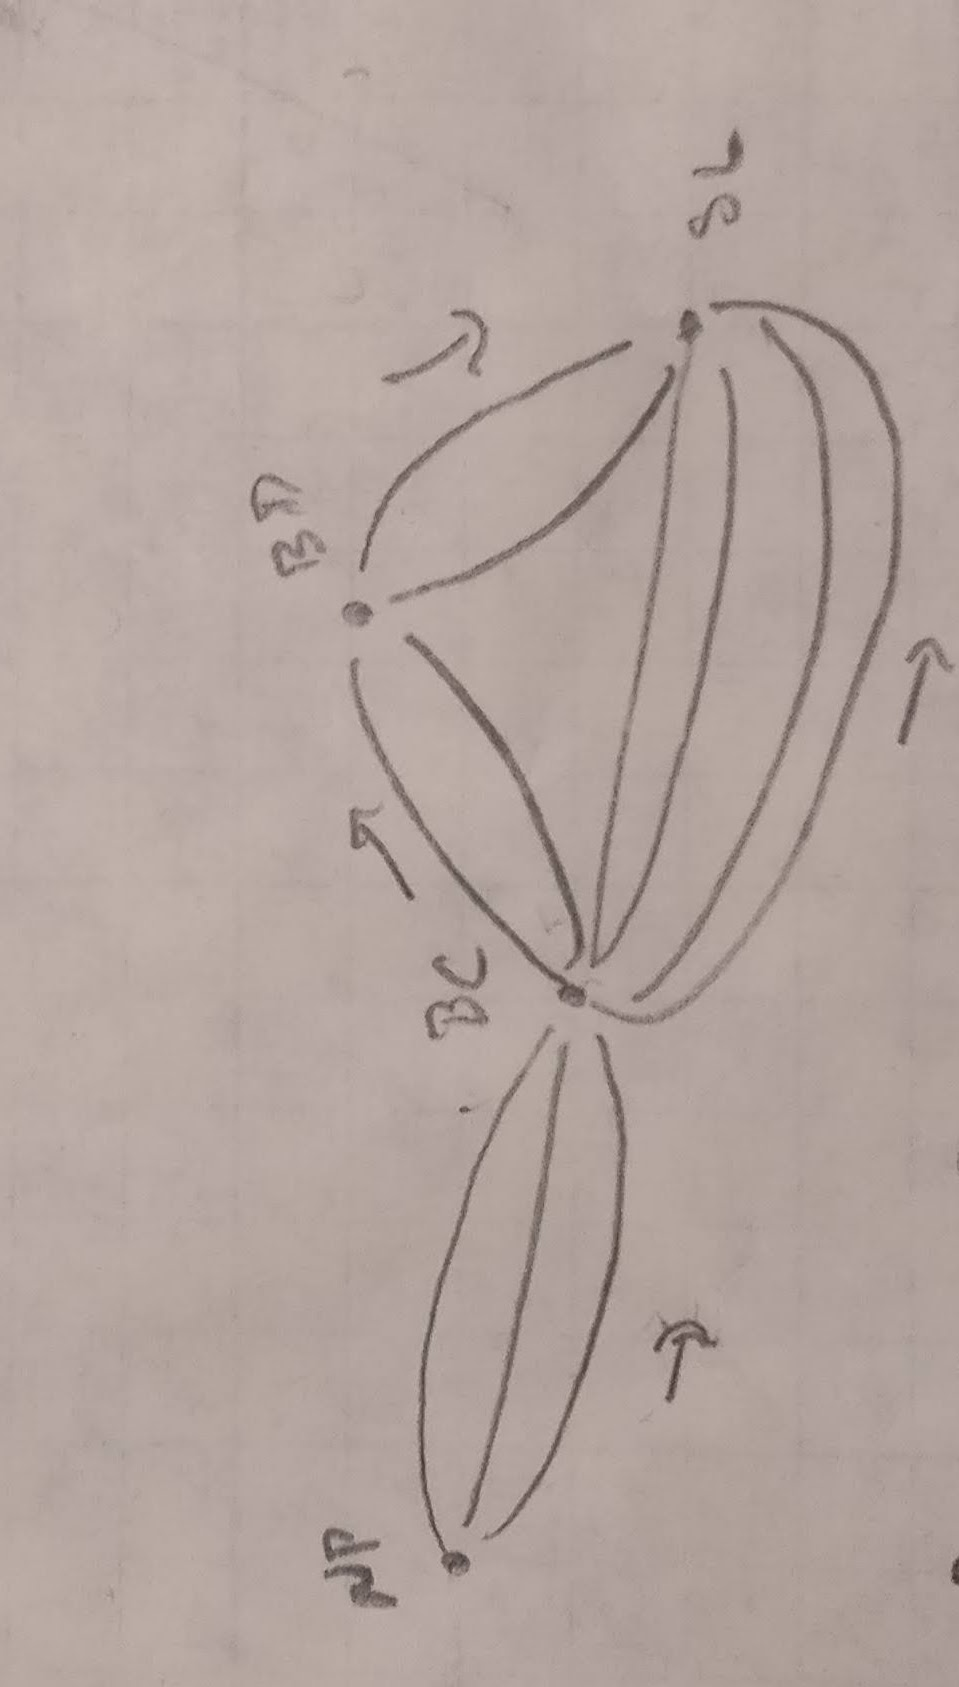
\includegraphics[width=8cm, angle=-90, scale=0.5]{map_image}}
\end{figure}

\section*{Section 9.2, Problem 10}
\begin{enumerate}[(a)]
	\item Question: How many paths are there from North Point to Star Lake that pass through Beaver Dam?\\
	Proof: $3*2*2=12$
	\item Question: How many paths are there from North Point to Star Lake that bypass Beaver Dam?\\
	Proof: $3*4=12$
\end{enumerate}

\problem{1-5}
\collab{Kevin Browder}
\clearpage
\header

\section*{Section 9.6, Problem 7}
Question: Prove $\displaystyle \binom{n+3}{n+1}=\dfrac{(n+3)*(n+1)}{2}$
\\\\
Proof:
\begin{center}
	\begin{align*}
		\displaystyle \binom{n+3}{n+1}&=\dfrac{(n+3)*(n+1)}{2}\\
		\dfrac{(n+3)!}{(n+1)!*((n+3)-(n+1))!}&=\\
		\dfrac{(n+3)*(n+2)*\cancel{(n+1)!}}{\cancel{(n+1)!}*2!}&=\\
		\dfrac{(n+3)*(n+1)}{2}&=\dfrac{(n+3)*(n+1)}{2}
	\end{align*}
\end{center}

\problem{1-6}
\collab{Kevin Browder}
\clearpage
\header

\section*{Section 9.6, Problem 32}
Question: Find the coefficient of $u^{16}*v^4$ in $(u^2-v^2)^{10}$
\\\\
Proof: Let $p=u^2$ and $q=v^2$ so $u^{16}*v^4=p^8*q^2$ binomial reads:
\begin{center}
	$(p-q)^{10}$
\end{center}
The binomial theorem is $\displaystyle \binom{n}{k}*a^{n-k}*b^k$ where $a^{n-k}*b^k=p^8*q^2$. Therefore, $k=2$ and $n-k=n-2=8$ which leads to $n=10$. The formula for the coefficient is given by $\displaystyle \binom{n}{k}$:
\begin{center}
	$\displaystyle\ \binom{10}{2}$\\
	$\dfrac{10!}{2!*(10-2)!}$\\
	$\dfrac{10*9*\cancel{8!}}{2!*\cancel{8!}}$\\
	$45$
\end{center}
The coefficient of $u^{16}*v^4$ is 45.

\problem{1-7}
\collab{none}
\clearpage
\header

\section*{Blaise Pascal and Computer Science}
Blaise Pascal was a French mathematician in the 1600s who is famous for publishing Pascal's Triangle and connecting it to the coefficients of Binomials. According to the Encyclopedia Britannica, Pascal "laid the foundations for the calculus of probabilities \cite{Britannica}." Pascal and his triangle relate closely to the Binomial Theorem, which we have already used in this class and will continue to use in computer science.

\newpage
\begin{thebibliography}{9}
	\bibitem{Britannica} The Editors of Encyclopedia Britannica "Blaise Pascal." Encyclopedia Britannica. Encyclopedia Britannica Inc., Aug 15, 2018. Britannica. Web. Sep 11, 2018.
\end{thebibliography}

\end{document}

